\documentclass{ieeeaccess}

\usepackage{cite}
\usepackage{amsmath,amssymb,amsfonts}
\usepackage{graphicx}
\usepackage{textcomp}
\usepackage{booktabs}
\usepackage{multirow}
\usepackage{array}
\usepackage{bm}
\usepackage{url}
\usepackage{algorithm}
\usepackage{algpseudocode}

\makeatletter
\AtBeginDocument{\DeclareMathVersion{bold}
\SetSymbolFont{operators}{bold}{T1}{times}{b}{n}
\SetSymbolFont{NewLetters}{bold}{T1}{times}{b}{it}
\SetMathAlphabet{\mathrm}{bold}{T1}{times}{b}{n}
\SetMathAlphabet{\mathit}{bold}{T1}{times}{b}{it}
\SetMathAlphabet{\mathbf}{bold}{T1}{times}{b}{n}
\SetMathAlphabet{\mathtt}{bold}{OT1}{pcr}{b}{n}
\SetSymbolFont{symbols}{bold}{OMS}{cmsy}{b}{n}
\renewcommand\boldmath{\@nomath\boldmath\mathversion{bold}}}
\makeatother

\graphicspath{{figures/}}

\newcommand{\ArxivShortSpeedup}{41.9}
\newcommand{\ArxivShortFullQ}{0.886}
\newcommand{\ArxivShortLocalQ}{0.881}
\newcommand{\ArxivShortQGap}{0.005}
\newcommand{\ArxivLongSpeedup}{30.5}
\newcommand{\ArxivLongFullQ}{0.887}
\newcommand{\ArxivLongLocalQ}{0.874}
\newcommand{\ArxivLongQGap}{0.013}
\newcommand{\ArxivLongFullNMI}{0.427}
\newcommand{\ArxivLongLocalNMI}{0.355}
\newcommand{\DSBMHighRandomSpeedup}{0.89}
\newcommand{\DSBMHighHubSpeedup}{0.85}
\newcommand{\PubMedTopologyQ}{0.7834}
\newcommand{\PubMedTopologySpeedup}{94.5}
\newcommand{\ArxivTopologyQ}{0.8787}
\newcommand{\ArxivTopologySpeedup}{634.3}


\begin{document}

% Production metadata are assigned by IEEE after acceptance.
\history{}
\doi{}
\vol{}
\year{}

\title{ComNetX: Local Hierarchical Adaptation for Batched Dynamic Community Detection}

\author{\uppercase{Aleksandr Konovalov}\authorrefmark{1},
\uppercase{Anna Uporova}\authorrefmark{1},
\uppercase{Alexander Drobyshev}\authorrefmark{1},
\uppercase{Iaroslav Egorov}\authorrefmark{1}, and
\uppercase{Grigoriy Bokov}\authorrefmark{1}}

\address[1]{AI Research Center, Lomonosov Moscow State University,
1 Leninskie Gory, Moscow 119991, Russian Federation}

\tfootnote{This work was supported by the Ministry of Economic Development of
the Russian Federation under subsidy agreement 000000C313925P4H0002, Grant
139-15-2025-012.}

\markboth
{Konovalov \headeretal: ComNetX: Local Hierarchical Adaptation for Batched Dynamic Community Detection}
{Konovalov \headeretal: ComNetX: Local Hierarchical Adaptation for Batched Dynamic Community Detection}

\begin{abstract}
Dynamic community detection is commonly addressed either by rerunning a static
detector on every snapshot or by developing an incremental procedure tied to a
particular optimizer. Full recomputation repeatedly processes unchanged graph
regions, whereas detector-specific procedures are difficult to transfer across
objectives, feature representations, and implementations. Localizing only by
graph distance creates a second problem: a small neighborhood may omit the
community context needed to revise a partition. We present ComNetX, a
hierarchical adaptation method that gives compatible partition-producing
detectors a common batched-update path. ComNetX expands the updated endpoints,
includes every vertex of each touched stored community, represents the
remaining hierarchy-defined groups as weighted supernodes, and invokes the
detector on a sequence of quotient graphs. The interface accepts aggregated
features for compatible feature-aware backends. Parent-quotient updates
preserve fine-to-coarse hierarchy nesting, while each quotient preserves
modularity within its induced atom-constrained search space. Update cost
depends on neighborhood reach, touched-community size, quotient size, and
backend cost. We evaluate ComNetX
on six real-graph update streams, two 500-update trajectories, multiple backends and design
controls, and DSBM stress streams with five graph seeds per condition. With
Leiden, ComNetX reduces cumulative measured processing time on all six short
streams. On arxivmath, it achieves a \ArxivShortSpeedup-fold speedup while
final modularity changes from \ArxivShortFullQ\ to \ArxivShortLocalQ; after
500 updates, the speedup remains \ArxivLongSpeedup-fold, with final modularity
\ArxivLongLocalQ\ versus \ArxivLongFullQ. For high-rate random and
hub-centered updates, full recomputation is faster.
\end{abstract}

\begin{keywords}
community detection, dynamic graphs, graph clustering, hierarchical graph
contraction, incremental graph analytics
\end{keywords}

\titlepgskip=-21pt
\maketitle

\section{Introduction}
\label{sec:introduction}
\PARstart{M}{any} communication, social, information, and collaboration
systems are represented by networks whose edges evolve over time
\cite{Onnela2007,Palla2007,Rossetti2018}. Community detection seeks groups of
vertices with coherent structural or functional roles
\cite{Porter2009,Fortunato2010,Radicchi2004,Flake2002}. The appropriate notion
of a community depends on the objective and on whether the analysis uses
topology, node attributes, temporal consistency, or a combination of these
signals \cite{Fortunato2016,Chunaev2020}. Modularity remains a widely used
structural criterion \cite{Newman2004,Brandes2008}; Louvain and Leiden are
widely used optimizers \cite{Blondel2008,Traag2019}, and parallel
implementations make them effective static baselines
\cite{Lu2015,Sahu2024FastLeiden}. In a dynamic setting, however, applying the
same optimizer after every batch keeps the update cost tied to the full graph,
even when the structural change is local.

Existing methods follow two main strategies. Full-snapshot recomputation reuses
a static implementation and may initialize it with the previous partition, but
it still processes the full graph. Incremental and dynamic algorithms instead
update selected parts of the previous solution
\cite{Halappanavar2017,Zhuang2021DynaMo,Zarayeneh2021DeltaScreening,
Sahu2025Dynamic}. Their speed comes from localization and refinement rules tied
to a particular objective, optimizer, or data structure, which makes the
methods difficult to reuse. This limitation is especially relevant to
attributed and representation-learning approaches, whose backend calls may
also construct features or perform iterative training
\cite{Tsitsulin2023DMoN,Liu2024MAGI,Lin2025S2CAG}. Reimplementing a distinct
dynamic algorithm for every such backend is costly and complicates controlled
comparison.

The central difficulty is not merely to find a small affected neighborhood,
but to retain enough of the current partition for the detector to reconsider
its decisions. A radius-limited subgraph can truncate communities at its
boundary; closing the neighborhood over every intersected community restores
its complete membership but may produce a large working graph. ComNetX separates the
scope of reassignment from the size of the problem presented to the detector.
Community closure determines which memberships may change, whereas a
hierarchy-defined atom partition compresses the same scope into a weighted
quotient. The detector is invoked through its existing partitioning interface,
and its output is lifted to the original vertices. The construction leaves the
backend implementation unchanged, but it remains a local approximation to
full-snapshot optimization: contracted atoms cannot split, and edges crossing
the selected scope are absent from the backend instance.

This separation is useful only when contraction removes enough detector work
to offset neighborhood search, closure, aggregation, projection, and data
conversion. On the reported streams, ComNetX with Leiden is faster in all six
short comparisons, reaching a \ArxivShortSpeedup-fold speedup on arxivmath
with an absolute final-modularity difference of \ArxivShortQGap. A separate
profile on the same graph closes over 41.95\% of the vertices but contracts the
final backend input to 0.23\%. Over 500 updates, the speedup remains
\ArxivLongSpeedup-fold; controlled synthetic streams show that the advantage
disappears when high-rate updates are random or concentrated around hubs.

The contributions of this work are as follows.

\begin{enumerate}
\item We introduce ComNetX, which converts each update batch into community
scopes computed from the immutable pre-update hierarchy and then into
hierarchy-aware weighted quotient graphs. It
reuses a compatible partition-producing detector without modifying its
implementation; the interface accepts topology-only inputs and aggregated
features for compatible feature-aware backends.
\item We show that successive parent-quotient updates preserve hierarchy
nesting and that, for atom-respecting partitions, each weighted quotient has
exactly the modularity of its lifted partition on the corresponding induced
scope. The worst-case time and memory bounds make explicit the dependence on
endpoint reach, touched-community size, quotient size, and backend cost.
\item The evaluation spans six real-graph update streams, two 500-update
trajectories, topology-only, feature-aware, and native dynamic backends,
component controls, and DSBM stress streams with five graph seeds per condition.
The largest time reductions occur with compact quotients and expensive full
calls; high-rate random or hub-centered updates and efficient native dynamic
state remove the advantage.
\end{enumerate}

\section{Related Work}
\label{sec:related}

\subsection{Static Objectives and Scalable Optimization}

Structural community definitions include dense-subgraph, cut-based,
information-flow, and null-model views \cite{Porter2009,Fortunato2010,
Radicchi2004}. Modularity compares within-community edge weight with a
degree-preserving null model \cite{Newman2004,Brandes2008}. Louvain combines
local moves with graph aggregation \cite{Blondel2008}; Leiden adds a refinement
stage that addresses poorly connected communities \cite{Traag2019}.
Shared-memory heuristics and fast Leiden variants extend this family to large static
graphs \cite{Lu2015,Sahu2024FastLeiden}. Other scalable perspectives include
the map-equation formulation of Infomap \cite{Rosvall2007}, fast label
propagation \cite{Traag2023LabelPropagation}, greedy modularity disassembly
\cite{Rustamaji2024}, and iterated local moves \cite{Taibi2025FLMIG}.

No single score fully determines whether a partition is useful. Modularity has
resolution effects and a highly degenerate optimization landscape
\cite{Good2010,Fortunato2016}; comparative studies also show that algorithm
rankings depend on the planted structure and evaluation design
\cite{Yang2016Comparative}. Class labels or other metadata may describe a
different organizing principle from graph structure
\cite{Yang2015GroundTruth,Peel2017}. We therefore report structural quality and
agreement with reference labels separately, using normalized mutual information
(NMI) as an external agreement measure \cite{Danon2005}.

\subsection{Dynamic, Temporal, and Local Community Detection}

Dynamic community detection spans evolutionary objectives, incremental
partition maintenance, and continuous-time models \cite{Rossetti2018}.
Snapshot-based methods reduce recomputation through incremental batch
processing \cite{Chong2013}, label propagation
\cite{Shang2014Realtime,Ma2020IncrementalLP,Seifikar2020,Xie2013LabelRankT,
Han2017AdaptiveLP}, incremental modularity optimization
\cite{Zhuang2021DynaMo}, or screened local moves
\cite{Zarayeneh2021DeltaScreening}. Scalable realizations include Grappolo,
DF-Louvain, multicore dynamic methods, and distributed DyG-DPCD
\cite{Halappanavar2017,Sahu2024DFLouvain,Sahu2025Dynamic,Sattar2025DyGDPCD};
broader algorithmic and parallel perspectives are surveyed in
\cite{Sattar2023,Hanauer2022DynamicGraphs}. In each case, locality is encoded in
method-specific state and update rules.

Other formulations make temporal persistence part of the objective. NOME
balances snapshot quality and temporal smoothness \cite{Cai2023NOME}; flow
stability, Matthew-effect models, and modularity-based tracking likewise model
temporal continuity \cite{Bovet2022FlowStability,Sun2022Matthew,Mazza2023}.
Continuous-time L-modularity avoids choosing snapshot boundaries
\cite{Brabant2025LModularity}, while recent work addresses sparse temporal
observations and random-walk snapshot clustering
\cite{Conrad2025Sparse,Blaskovic2025}. ComNetX instead targets batched snapshot
maintenance through a reusable partitioning interface and returns a complete
partition after every batch.

The term \emph{local} also covers a different output contract. Seed-, query-,
and anchor-based methods find one or several nearby communities rather than a
partition of every vertex \cite{DiTursi2017,Christopoulos2023,
Liu2021MultiLocal}. OLCPM maintains overlapping communities online
\cite{Boudebza2018OLCPM}. ComNetX preserves a complete label vector and holds
labels outside the closed update scope fixed. It therefore uses locality to
maintain a full partition rather than to change the output contract.

\subsection{Attributed and Representation-Learning Methods}

Attributed community detection combines topology with node information
\cite{Chunaev2020}. Message-passing graph neural networks provide a general
representation framework \cite{Scarselli2009}; later community-oriented
methods include SEAL \cite{Zhang2020SEAL}, DMoN
\cite{Tsitsulin2023DMoN}, CommDGI \cite{Zhang2020CommDGI}, MAGI
\cite{Liu2024MAGI}, and DGCluster \cite{Bhowmick2024DGCluster}. Comparative
and survey work documents the range of embeddings, clustering losses, and
evaluation choices \cite{Kumar2024GNNStudy,Liu2026DeepGraphSurvey}. DAG learns
clusters without a prescribed cluster count \cite{Liu2024DAG};
structural-entropy objectives provide another unsupervised signal
\cite{Zhang2025StructuralEntropy}; and fairness-aware formulations introduce
constraints beyond aggregate clustering quality \cite{Gkartzios2025Fair}.

Efficiency-oriented designs include pre-train-and-refine community detection
and inductive graph partitioning \cite{Qin2024PretrainRefine,Qin2024PRGPT},
while Spectral Subspace Clustering for Attributed Graphs (S$^2$CAG) provides a
feature-aware spectral approach \cite{Lin2025S2CAG}. Community structure can
also be part of a downstream
dynamic prediction model \cite{Ji2023DynamicPopularity}. MFC combines matrix
factorization with a topological regularizer to learn persistent communities
\cite{Kong2024MFC}. For compatible partition-producing feature-aware backends,
ComNetX supplies a contracted adjacency and aggregated group features. The
fixed-budget
S$^2$CAG experiments in Section~\ref{sec:backend_results} evaluate this
feature-aware interface alongside topology-only and native dynamic calls.
Because contraction and feature aggregation change the input representation,
interface compatibility does not imply preservation of a feature-aware
objective.

\subsection{Difference from Existing Local and Dynamic Methods}

Dynamic methods obtain locality at different layers. Solver-specific methods
restrict moves, refinement steps, or state transitions inside a particular
optimizer. LD-Leiden, for example, repairs a Leiden partition locally and
exploits shared-memory parallelism
\cite{Bokov2026LDLeiden}; HIT-Leiden maintains connected-component and
hierarchical state to bound the affected range \cite{Lin2026HITLeiden}; and
Sahu et al. develop a separate Leiden-specific
update path \cite{Sahu2024Start}. Seed- and
anchor-local methods instead reduce computation by returning selected
communities. ComNetX retains the full-partition output contract but localizes
the graph presented to the backend. It expands an updated neighborhood to
include complete current communities and contracts groups defined by the
stored hierarchy. It can therefore reuse a static or feature-aware partitioner
without implementing backend-specific update rules, at the cost of discarding
any persistent backend state. A specialized dynamic solver can be used as a
ComNetX backend only if it can independently partition each supplied quotient
graph; DF-Leiden used in this way is reinitialized on every quotient and is not
equivalent to its native streaming mode.

\section{Problem Formulation}
\label{sec:problem}

\subsection{Batched Graph Model}

Let $G_t=(V,E_t,\bm{A}_t,\bm{X})$ be the graph after batch $t$, with a fixed
vertex set $V$, $n=|V|$, sparse adjacency $\bm{A}_t$, and optional node-feature
matrix $\bm{X}\in\mathbb{R}^{n\times d}$. A sparse signed batch $\bm{\Delta}_t$
updates the stored adjacency as
\begin{equation}
\bm{A}_t=\bm{A}_{t-1}+\bm{\Delta}_t.
\label{eq:update}
\end{equation}
Its directly affected vertices are
\begin{equation}
S_t=\{i:\exists j,\ \Delta_t(i,j)\ne0\ \text{or}\
\Delta_t(j,i)\ne0\}.
\label{eq:affected}
\end{equation}
This fixed-vertex model accepts signed sparse batches. The experiments focus on
edge-insertion streams with fixed attributes, which isolate the cost of batched
structural updates.

We treat a community-detection backend as a partition-producing procedure
\begin{equation}
\mathcal{B}(\bm{A},\bm{X},\bm{y}_0;\bm{\theta})\longmapsto\bm{y},
\label{eq:backend}
\end{equation}
where $\bm{X}$ and the initial partition $\bm{y}_0$ are optional, and
$\bm{\theta}$ denotes backend-specific settings such as resolution or a fixed
iteration budget. For an input of $m$ vertices, the interface requires one
integer label per input vertex; equality of labels defines the returned
partition, while their numerical values and ordering are immaterial. This
contract covers modularity heuristics and attributed clustering methods. It
also covers a native dynamic implementation when that implementation can be
called independently on each supplied graph and returns one label per input
vertex. ComNetX does not reuse backend state between its quotient calls; each
backend retains its own objective and optimization procedure.

Full-snapshot recomputation at update $t$ invokes $\mathcal{B}$ on $\bm{A}_t$.
When the backend accepts an initialization, the previous partition is supplied:
\begin{equation}
\bm{y}^{\mathrm{full}}_t=
\mathcal{B}(\bm{A}_t,\bm{X},\bm{y}_{t-1};\bm{\theta}).
\label{eq:full_backend}
\end{equation}
The full Leiden baseline follows this warm-started definition. The
ComNetX state instead comprises the resident sparse adjacency, optional full
feature matrix, and $L$ full-length label vectors used to construct the local
problems described next.

\subsection{Quality Metrics and Timing}

All main comparisons use an undirected graph representation. Sources marked as
directed are symmetrized within the paired full/local experiment, and a
separate control retains direction. For a weighted adjacency, let
$W=\sum_{i,j}A_{ij}$,
$d_i^{\mathrm{out}}=\sum_jA_{ij}$, and
$d_j^{\mathrm{in}}=\sum_iA_{ij}$. We compute directed modularity at resolution
$\gamma$ as
\begin{equation}
Q_\gamma(C)=\frac{1}{W}\sum_{i,j}
\left(A_{ij}-\gamma\frac{d_i^{\mathrm{out}}d_j^{\mathrm{in}}}{W}\right)
\mathbf{1}\{C(i)=C(j)\},
\label{eq:modularity}
\end{equation}
which reduces to the standard undirected expression when $\bm{A}$ is symmetric,
$W=2m$, and $d_i^{\mathrm{out}}=d_i^{\mathrm{in}}=d_i$. The main experiments
use $\gamma=1$ unless a resolution sweep is stated. We also use normalized
mutual information (NMI),
\begin{equation}
\operatorname{NMI}(C,Z)=\frac{2I(C;Z)}{H(C)+H(Z)},
\label{eq:nmi}
\end{equation}
between partition $C$ and reference class labels $Z$
\cite{Danon2005}. These labels are metadata, not asserted structural ground
truth \cite{Peel2017}.

The principal efficiency measure is cumulative processing time within the
stated measurement interval. For ComNetX, this interval includes
neighborhood expansion, closure, adjacency restriction, contraction, backend
calls, and projection. It excludes initial partition construction, application
of the sparse update to the resident adjacency, metric evaluation, data loading,
and backend-format conversion. Speedup is the full or native-dynamic time
divided by ComNetX time under the same paired definition.

The component comparison uses a broader profile clock. It includes
adjacency-update time and the interval from neighborhood expansion through projection,
including backend-format conversion. The separately timed boundary diagnostic
is excluded. Applying the same definition to all three variants makes their
times directly comparable.

\section{ComNetX Method}
\label{sec:method}

\subsection{Update Procedure and Stored State}

ComNetX separates three aspects of a local update: the vertices eligible for
relabeling, the indivisible groups that define the local search space, and the
graph presented to the backend. The closed scope $U_t^\ell$ controls the first,
the atom partition $\mathcal{G}_t^\ell$ controls the second, and the quotient
$\bar{\bm A}_\ell$ realizes the resulting compact backend problem. All scopes are fixed from the immutable
pre-update hierarchy before the levels are processed. The method is implemented
as an adapter around a partition-producing backend $\mathcal{B}$: it constructs
one reduced graph per level, invokes $\mathcal{B}$, and projects the returned
partition to the original vertices. Fig.~\ref{fig:pipeline} shows the complete
update.

The maintained state consists of the accumulated sparse adjacency $\bm{A}_t$,
the optional feature matrix $\bm{X}$, and the full-length integer label tensor
$\bm{C}_t=(C_t^0,\ldots,C_t^{L-1})$. Let
$\mathcal{P}_t^\ell$ denote the partition induced by $C_t^\ell$, and write
$\mathcal{P}\preceq\mathcal{Q}$ when $\mathcal{P}$ refines $\mathcal{Q}$. We use the
visual order in Fig.~\ref{fig:pipeline}: $C_t^0$ is the coarsest level and
$C_t^{L-1}$ is the finest, reported partition. Thus every block of
$\mathcal{P}_t^{\ell+1}$ is contained in a block of
$\mathcal{P}_t^\ell$.

Every stored block $H$ is represented canonically by
$\kappa(H)=\min H$. Canonical labels are deterministic original-vertex indices
and, unlike raw backend labels, cannot collide for disjoint blocks. At
initialization, a designated full-graph method produces
$\mathcal{P}_0^{L-1}$; the experiments use Leiden for this initialization,
including experiments with other local backends. Each next coarser level
partitions an exact quotient
whose vertices are the blocks of the preceding finer level, and its labels are
lifted to $V$. The initial hierarchy is therefore nested, although adjacent
levels need not be distinct. Only $C_t^{L-1}$ is reported as the current
community assignment; the other rows retain the parent structure needed by
later updates.

\begin{figure*}[t]
\centering
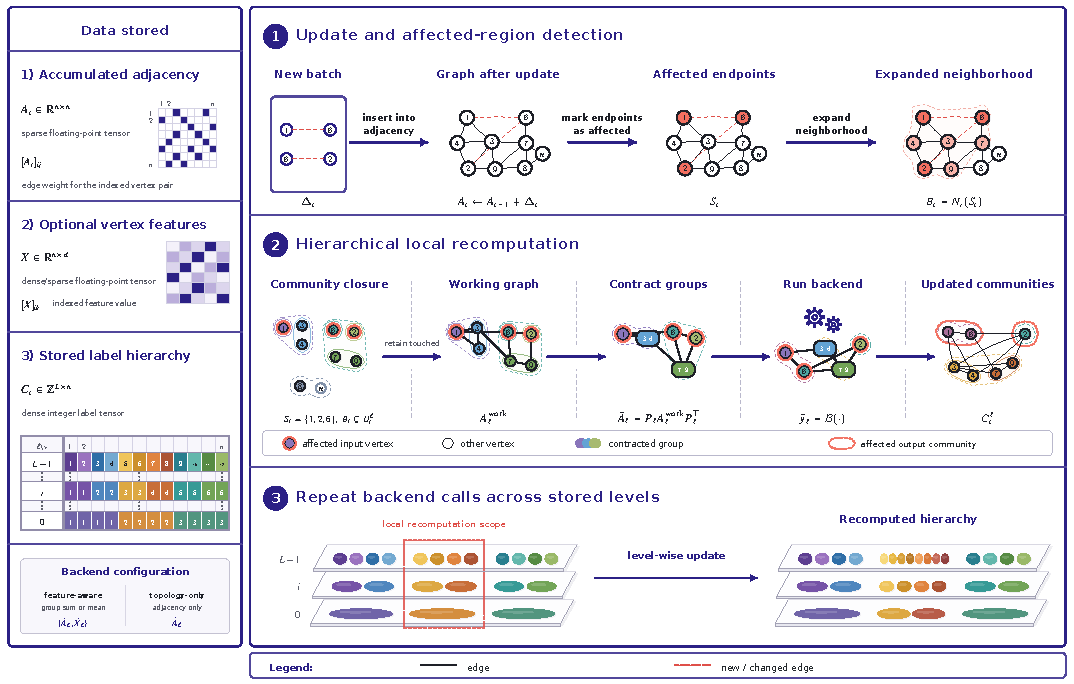
\includegraphics[width=\textwidth]{method_pipeline.pdf}
\caption{ComNetX update procedure. The endpoints of a new batch are expanded
to a local neighborhood, and each level-specific region includes every
pre-update community that intersects this neighborhood. These regions are
fixed before any partition is changed. Passes proceed from the finest reported
level $C_t^{L-1}$ to the coarsest level $C_t^0$. Each pass contracts a fresh
induced graph; after the first pass, each quotient vertex is a complete block
of the already updated finer partition. Backend labels are mapped to the
original vertices and replaced by canonical labels, while labels outside the
corresponding region remain unchanged.}
\label{fig:pipeline}
\end{figure*}

\subsection{Selecting the Communities to Recompute}

After applying a batch, ComNetX expands $S_t$ by $r$ hops on the support of
$\bm{A}_t+\bm{A}_t^{\mathsf T}$. The resident adjacency is assumed
nonnegative after the signed batch has been applied, as it is in the evaluated
insertion streams; under this condition the sparse matrix--vector traversal
equals reachability on the symmetrized support. Let
\begin{equation}
B_t=N_r(S_t)=\{v:\operatorname{dist}(v,S_t)\le r\}.
\label{eq:radius}
\end{equation}
Before any hierarchy row is modified, one scope is computed at every level
from the immutable pre-update state:
\begin{equation}
U_t^\ell=\{v:C_{t-1}^\ell(v)\in
C_{t-1}^\ell(B_t)\},\qquad 0\le\ell<L.
\label{eq:closure}
\end{equation}
Hence $U_t^\ell$ is the union of all pre-update level-$\ell$ communities that
meet $B_t$.

This closure is the smallest union of complete
$\mathcal{P}_{t-1}^\ell$-blocks containing $B_t$. Because the stored
partitions are nested, the corresponding scopes are nested as well,
\begin{equation}
B_t\subseteq U_t^{L-1}\subseteq U_t^{L-2}\subseteq\cdots\subseteq U_t^0.
\label{eq:nested_closures}
\end{equation}
A fine block meeting $B_t$ lies in a coarse block that also meets $B_t$.
Closure therefore restores the complete membership of each touched community
without performing another graph-distance expansion.

\subsection{Finest-Level Atoms and Coarser Parent Quotients}

The first pass, at the reported level $L-1$, uses the base atoms
\begin{equation}
\begin{aligned}
\mathcal{G}_t^{L-1}={}&\{\{v\}:v\in B_t\}\\
&{}\cup\bigl\{(H\cap U_t^{L-1})\setminus B_t:
H\in\mathcal{P}_{t-1}^{0},\\
&\hspace{34mm}(H\cap U_t^{L-1})\setminus B_t\ne\varnothing\bigr\}.
\end{aligned}
\label{eq:base_atoms}
\end{equation}
Every radius-expanded vertex is therefore represented by a singleton atom,
whereas the remaining scoped vertices retain the grouping supplied by their
pre-update coarsest community.
For each subsequent, coarser pass $\ell<L-1$, the atoms are precisely the
complete blocks of the already updated finer partition within its larger
scope:
\begin{equation}
\mathcal{G}_t^\ell=
\{H\in\mathcal{P}_t^{\ell+1}:H\subseteq U_t^\ell\}.
\label{eq:parent_atoms}
\end{equation}

Every pass starts from a fresh restriction of the resident adjacency,
\begin{equation}
\bm{A}^{\mathrm{work}}_\ell=\bm{A}_t[U_t^\ell],
\label{eq:u0adj}
\end{equation}
where rows and columns outside $U_t^\ell$ are absent or equivalently zero in
the ambient $n\times n$ representation. No edge deletion from a preceding
pass is carried forward. If $k_\ell=|\mathcal{G}_t^\ell|$, the membership
matrix $\bm{P}_\ell\in\{0,1\}^{k_\ell\times n}$ contains one unit entry in
each column indexed by $U_t^\ell$ and zero columns outside the scope. The
backend adjacency is
\begin{equation}
\bar{\bm{A}}_\ell=\bm{P}_\ell
\bm{A}^{\mathrm{work}}_\ell\bm{P}_\ell^{\mathsf T}.
\label{eq:aggregate}
\end{equation}
The backend therefore receives one vertex per atom and the total weight
between every ordered pair of atoms.

For a feature-aware backend, ComNetX supports sum and mean aggregation. For
$G_{\ell a}\in\mathcal{G}_t^\ell$,
\begin{equation}
\bar{\bm{x}}_{\ell a}=
\begin{cases}
\displaystyle\sum_{i\in G_{\ell a}}\bm{x}_i,
&\text{sum},\\[1mm]
\displaystyle\frac{1}{|G_{\ell a}|}
\sum_{i\in G_{\ell a}}\bm{x}_i,
&\text{mean}.
\end{cases}
\label{eq:features}
\end{equation}

\noindent\textbf{Proposition 1 (exact scoped quotient):} Write
$Q_\gamma(\bm A,c)$ for \eqref{eq:modularity} evaluated on adjacency $\bm A$.
Let $\bm A_U\in\mathbb{R}^{|U|\times|U|}$ be the locally indexed adjacency
induced by one working scope, assume its total weight $W_U$ is positive, and
let $\mathcal{G}=\{G_1,\ldots,G_k\}$ be a partition of $U$. Define the local
membership matrix $\bm P_U\in\{0,1\}^{k\times|U|}$ and let
$\bar{\bm A}=\bm P_U\bm A_U\bm P_U^{\mathsf T}$, retaining the self-loops
created by aggregation. Then
\begin{equation}
\bar A_{ab}=\sum_{i\in G_a}\sum_{j\in G_b}A_{ij}.
\label{eq:quotient_entries}
\end{equation}
Consequently, the quotient preserves total weight and the sums of outgoing and
incoming weighted degrees. Every quotient partition $z$ induces a unique
atom-constant partition $c$ of $U$, and, under the same directed or symmetric
adjacency, self-loop, and resolution conventions,
\begin{equation}
Q_\gamma(\bar{\bm A},z)=Q_\gamma(\bm A_U,c).
\label{eq:quotient_modularity}
\end{equation}
The identity follows by expanding each quotient entry in the internal-weight
and degree terms of \eqref{eq:modularity}. Hence contraction preserves
modularity exactly within the atom-constant search space of the induced working
graph. This identity does not cover atom splits, omitted boundary edges, or
arbitrary feature-aware objectives.

The current implementation calls the backend without an initial quotient
partition: the stored hierarchy determines the atoms but is not passed as
$\bm y_0$. After the backend returns a quotient label vector, its induced blocks are
lifted through $\bm P_\ell$. Each lifted block $H\subseteq U_t^\ell$ receives
the canonical label $\kappa(H)=\min H$; labels outside $U_t^\ell$ remain
unchanged. Algorithm~\ref{alg:comnetx} summarizes one batch update.

\begin{algorithm}[t]
\caption{ComNetX update for one batch}
\label{alg:comnetx}
\begin{algorithmic}[1]
\Require $\bm{A}_{t-1}$, $\bm{C}_{t-1}$, optional $\bm{X}$, update
$\bm{\Delta}_t$, radius $r$, backend $\mathcal{B}$, settings $\bm\theta$
\State $\bm{A}_t\gets\bm{A}_{t-1}+\bm{\Delta}_t$
\State $S_t\gets$ endpoints of the updated edges; $B_t\gets N_r(S_t)$
\For{$\ell=0,\ldots,L-1$}
    \State $U_t^\ell\gets$ closure of $B_t$ under
    $\mathcal{P}_{t-1}^\ell$ \Comment{immutable}
\EndFor
\State $\bm{C}_t\gets\bm{C}_{t-1}$
\For{$\ell=L-1,\ldots,0$}
    \If{$\ell=L-1$}
        \State $\mathcal{G}_t^\ell\gets$ radius-expanded singletons and nonempty
        coarsest-block remainders in \eqref{eq:base_atoms}
    \Else
        \State $\mathcal{G}_t^\ell\gets$ complete updated
        $\mathcal{P}_t^{\ell+1}$-blocks in $U_t^\ell$
    \EndIf
    \State $\bm{A}^{\mathrm{work}}_\ell\gets\bm{A}_t[U_t^\ell]$
    \State build $\bm{P}_\ell$ from $\mathcal{G}_t^\ell$
    \State $\bar{\bm{A}}_\ell\gets
    \bm{P}_\ell\bm{A}^{\mathrm{work}}_\ell\bm{P}_\ell^{\mathsf T}$
    \State aggregate $\bar{\bm{X}}_\ell$ if $\mathcal{B}$ uses features
    \State $\bar{\bm{y}}_\ell\gets
    \mathcal{B}(\bar{\bm{A}}_\ell,\bar{\bm{X}}_\ell,\varnothing;\bm\theta)$
    \State lift $\bar{\bm{y}}_\ell$ to $U_t^\ell$ and label each lifted
    block $H$ by $\min H$
\EndFor
\State \Return $\bm{C}_t$ with reported partition $C_t^{L-1}$
\end{algorithmic}
\end{algorithm}

\subsection{Hierarchy Consistency Across Levels}

Recomputing hierarchy levels independently can produce incompatible
partitions. ComNetX instead makes every updated finer block an indivisible atom
of the next coarser pass.

\noindent\textbf{Proposition 2 (hierarchy preservation under parent-quotient
updates):} Under Algorithm~\ref{alg:comnetx}, assume that the pre-update
hierarchy is canonical and nested, all scopes are computed before any partition
is modified, projection uses canonical labels while retaining the partition
outside each scope, and every coarser backend call treats the updated blocks of
the preceding finer level as indivisible atoms. Then the updated partitions
remain nested:
\begin{equation}
\mathcal{P}_t^{L-1}\preceq
\mathcal{P}_t^{L-2}\preceq\cdots\preceq\mathcal{P}_t^0.
\label{eq:hierarchy_nesting}
\end{equation}

Equation~\eqref{eq:nested_closures} places each updated finer scope inside the
corresponding coarser scope. Moreover, $U_t^\ell$ is a union of pre-update
level-$\ell$ blocks and therefore, by pre-update nesting, a union of complete
level-$(\ell+1)$ blocks. The finer pass changes only $U_t^{\ell+1}$; its lifted
blocks stay inside that scope, while canonical labels prevent them from
colliding with retained outside blocks. Since
$U_t^{\ell+1}\subseteq U_t^\ell$, the coarser scope remains a union of complete
updated level-$(\ell+1)$ blocks. Equation~\eqref{eq:parent_atoms} makes each of
these blocks one quotient vertex, so the coarser backend may merge but cannot
split it. Descending induction over $\ell$ gives
\eqref{eq:hierarchy_nesting}; the nesting can be non-strict when a backend
leaves adjacent levels equal.

Canonical labels also make projection invariant to backend label permutations:
disjoint lifted blocks receive distinct original-vertex identifiers. Retaining
labels outside $U_t^\ell$ yields a complete label vector after each pass.

\subsection{Relation to the Full-Graph Objective}

Proposition~1 applies to the induced working graph. A local backend does not
see edges crossing from $U_t^\ell$ to the rest of the graph, so its modularity
ranking need not equal the full-graph ranking. The exact decomposition in
Appendix~\ref{app:boundary} attributes this discrepancy to boundary degrees and
global-versus-local null-model normalization. We therefore evaluate every
returned partition on the full graph.

\subsection{Time and Memory Complexity}

For $r=1$, if $d_t(v)$ is degree in the symmetrized support graph, then
\begin{equation}
|B_t|\le |S_t|+\sum_{v\in S_t}d_t(v).
\label{eq:r1_bound}
\end{equation}
Thus, a small edge batch can still have a large radius-one expansion when it
touches hubs. If $\mathcal{P}_{t-1}^\ell$ is the pre-update level-$\ell$
partition, the closure size $h_\ell=|U_t^\ell|$ is exactly
\begin{equation}
h_\ell=\sum_{C\in\mathcal{P}_{t-1}^\ell:\,C\cap B_t\ne\varnothing}|C|.
\label{eq:closure_size}
\end{equation}
Thus batch size, endpoint degree, and touched-community size control different
stages. Let $r_t\le r$ be the number of neighborhood traversals, $s_t$ the
number of stored adjacency entries, $e_\ell$ the number of entries in
$\bm A_t[U_t^\ell]$, and $k_\ell$ and $q_\ell$ the numbers of quotient
vertices and entries. Let
$\overline T_{\mathcal B}(k,q,d)$ and
$\overline M_{\mathcal B}(k,q,d)$ be nondecreasing worst-case envelopes for
the core backend time and working memory, excluding format conversion. Assume
that conversion of a quotient to the backend representation is linear in its
stored adjacency and feature arrays; these terms are dominated below by the
quotient-construction and feature terms. The following bound assumes direct
endpoint relabeling and comparison-based sort-and-reduce; the current PyTorch
realization is analyzed separately below and in
Appendix~\ref{app:implementation_cost}.

\noindent\textbf{Proposition 3 (worst-case resources):} For a feature-aware
call, let $F=nd$, a valid upper bound for dense or sparse feature storage; for
a topology-only call, let $F=0$. Suppose quotient edges
are assembled by relabeling their endpoints followed by comparison-based
sort-and-reduce and levels are processed sequentially. After the batch has been
applied, one update can be implemented in
\begin{equation}
\begin{aligned}
T_{\mathrm{update}}=O\!\Bigl(&r_t(n+s_t)
+L\bigl[(n+s_t)\log(2+n+s_t)+F\bigr]\\
&{}+\sum_{\ell=0}^{L-1}\overline T_{\mathcal B}(k_\ell,q_\ell,d)\Bigr)
\end{aligned}
\label{eq:update_time_bound}
\end{equation}
time and
\begin{equation}
\begin{aligned}
M_{\mathrm{peak}}=O\!\Bigl(&s_t+Ln+F+\\
&\max_\ell\{e_\ell+h_\ell+q_\ell
+\overline M_{\mathcal B}(k_\ell,q_\ell,d)\}\Bigr)
\end{aligned}
\label{eq:peak_space_bound}
\end{equation}
memory. The maintained state alone occupies $O(s_t+Ln+F)$ memory. The time
bound follows from at most $r_t$ sparse traversals, $L$ scans of the label and
edge arrays, sort-and-reduce construction of at most $s_t$ quotient entries per
level, at most one feature aggregation and linear format conversion per level,
and the $L$ backend calls. The space bound follows because only one level,
converted quotient, and backend call need to be materialized at a time.

Since $h_\ell,k_\ell\le n$ and $e_\ell,q_\ell\le s_t$, a nondecreasing backend
cost gives the explicit graph-wide worst case
\begin{equation}
\begin{aligned}
T_{\mathrm{worst}}=O\!\Bigl(&r_t(n+s_t)+\\
&L\bigl[(n+s_t)\log(2+n+s_t)+F
+\overline T_{\mathcal B}(n,s_t,d)\bigr]\Bigr).
\end{aligned}
\label{eq:graph_wide_worst}
\end{equation}
Thus ComNetX has no unconditional asymptotic speedup: a hub-centered update or
a large touched community can make every local problem comparable to the full
snapshot, and up to $L$ backend calls are then required.

The present PyTorch implementation uses tensor sparse primitives rather than
the sort-and-reduce realization used for Proposition~3. It filters the full
resident edge array at every hierarchy level. Conditional on executing all
$r_t$ traversals and $L$ passes, it therefore incurs
\begin{equation}
\Omega\!\left(r_ts_t+L(n+s_t)\right)
\label{eq:full_scan_lower}
\end{equation}
full-scan memory traffic even when the quotient graphs are small. Its
primitive-level time and workspace accounting is given in
Appendix~\ref{app:implementation_cost}.

This full-scan cost is not required by the update rule. Maintaining adjacency,
community-member, and incident-edge indices can replace mandatory global scans
by work proportional to the reached regions, although index maintenance has its
own cost and the graph-wide worst case remains. Appendix~\ref{app:implementation_cost}
gives the corresponding output-sensitive bound.

Without a backend-specific cost model, local graph sizes do not imply a
speedup. Contraction pays only when the backend work eliminated by the quotient
calls exceeds neighborhood search, closure, restriction, aggregation,
projection, and format-conversion costs. The observable quantities $|B_t|$,
$h_\ell$, $e_\ell$, $k_\ell$, and $q_\ell$ are therefore workload indicators,
not a performance certificate.

\section{Experimental Design}
\label{sec:experiments}

We organize the evaluation around five questions.
\begin{enumerate}
\item[\textbf{RQ1}] What quality--time trade-off does ComNetX achieve relative
to warm-started full-snapshot recomputation?
\item[\textbf{RQ2}] How does this trade-off change with the wrapped backend,
including feature-aware calls under backend-specific interface rules and a
specialized dynamic implementation?
\item[\textbf{RQ3}] How do radius expansion and community closure change the
selected scope, and how far does quotient contraction reduce the final backend
input?
\item[\textbf{RQ4}] How does the measured quality--time behavior change when
closure or contraction is removed, and how sensitive is it to hierarchy depth,
radius, resolution, edge direction, and feature representation?
\item[\textbf{RQ5}] How does the trade-off evolve over long update sequences
and as the number and placement of changed edges vary?
\end{enumerate}

\subsection{Datasets and Stream Construction}

Table~\ref{tab:datasets} lists the six input graphs. Cora, ACM, Citeseer, and
PubMed are static attributed topologies converted into reproducible update
benchmarks with artificial edge orders. Patent and arxivmath use
timestamped sequences from temporal graph-clustering
resources \cite{Liu2025BenchTGC,Liu2023Arxiv4TGC}; their edges are sorted by
the provided timestamps and divided into equal-edge-count bins. The table
reports stored source edge counts before any required symmetrization.

\begin{table}[t]
\centering
\caption{Update-stream benchmarks and actual short-protocol updates.}
\label{tab:datasets}
\setlength{\tabcolsep}{2.2pt}
\scriptsize
\begin{tabular}{@{}lrrlc@{}}
\toprule
\textbf{Dataset} & \textbf{Vertices} & \textbf{Edges} &
\textbf{Order} & \textbf{Updates} \\
\midrule
dyn\_cora & 2,708 & 5,278 & stored artificial order & 10 \\
dyn\_acm & 3,025 & 13,128 & stored artificial order & 10 \\
dyn\_citeseer & 3,327 & 4,552 & stored artificial order & 8 \\
patent & 12,214 & 41,916 & timestamp order & 10 \\
dyn\_pubmed & 19,717 & 44,338 & stored artificial order & 10 \\
arxivmath & 270,013 & 799,745 & timestamp order & 10 \\
\bottomrule

\end{tabular}
\end{table}

A real-graph strategy $p{:}q$ partitions the stored sequence into $p+1$ coarse bins,
uses the first $p$ bins as the initial graph, and splits the tail bin into at
most $q$ equal edge chunks. Empty chunks are skipped. Thus $999{:}10$ produces
ten measured updates for five graphs but eight for dyn\_citeseer. The
$9{:}500$ protocol produces 500 updates on dyn\_pubmed and arxivmath. The short
protocol has five repeated executions for these two larger datasets and one
execution for each other dataset. Repetitions use the same stream and settings
to quantify timing repeatability.

Each dynamic stochastic block model (DSBM) sequence begins from a separately
stored initial snapshot; the
archive label $0{:}99$ denotes its 99 measured update batches rather than an
empty initial graph. The synthetic suite has $n=100{,}000$ vertices, 32 planted blocks, target
average degree 58, maximum configured degree 1024, and 1\% high-degree vertices
with target average degree 512. The low and high workloads modify 290 and 1450 edges per
update, respectively, under random, hub-centered, or community-internal
selection. Each condition uses five paired graph seeds, 42--46. The suite is
motivated by static and dynamic stochastic block models
\cite{Holland1983,Xu2014DSBM}; by varying both the number and placement of
updated edges, it tests when local recomputation remains faster than processing
the full graph.

Table~\ref{tab:protocols} lists the evaluation protocols. The strategies are
edge-sequence partitions rather than durations, and the actual
number of nonempty updates is reported instead of assuming that it equals the
requested maximum. A repeated run means another execution of the same retained
input; the DSBM suite additionally varies the graph seed.

\begin{table*}[t]
\centering
\caption{Evaluation protocols used in this study.}
\label{tab:protocols}
\setlength{\tabcolsep}{4.0pt}
\small
\begin{tabular}{@{}lllll@{}}
\toprule
\textbf{Purpose} & \textbf{Graphs} & \textbf{Strategy} &
\textbf{Actual updates} & \textbf{Replication} \\
\midrule
Main Leiden comparison & six real topologies & $999{:}10$ & 8--10 & five fixed-input runs on two graphs \\
Different backends & dyn\_pubmed, arxivmath & $999{:}10$ & 10 & five fixed-input runs \\
Topology and direction controls & selected real topologies & $999{:}10$ & 10 & single runs except the default point \\
Closure, contraction, and resolution & three/two real topologies & $999{:}50$ & 10, 44, or 50 & single runs \\
S$^2$CAG feature modes & dyn\_cora, dyn\_pubmed & $999{:}100$ & 10 or 44 & single fixed-budget runs \\
Long horizon & dyn\_pubmed, arxivmath & $9{:}500$ & 500 & one stream window \\
Synthetic stress & 30 DSBM streams & $0{:}99$ & 99 & five graph seeds per condition \\
\bottomrule
\end{tabular}
\end{table*}

All wall-clock measurements were collected on a Dockerized Linux server with
two AMD EPYC 7742 64-core central processing units (CPUs), 2.0 TiB of
random-access memory (RAM), and eight NVIDIA A100-SXM4 graphics processing
units (GPUs; 80 GB each). The NVIDIA driver was 535.216.03,
\texttt{nvidia-smi} reported
CUDA 12.2, and the container used Python 3.10.13, PyTorch 2.3.1 with CUDA 11.8,
and TensorFlow 2.14.0.

The component, cut-metric, direction, resolution, and feature controls use
separate paired experiments. Each control is interpreted within its stated
protocol and is not pooled with repetitions of the main comparison.

\subsection{Methods and Fixed Configuration}

Leiden is the primary backend and uses resolution 1. Full recomputation receives
the previous partition as a warm start. ComNetX uses $L=3$, $r=1$, and the
Leiden initialization described in Section~\ref{sec:method}. ComNetX quotient
calls are label-free: the hierarchy defines the contracted atoms but is not
passed to the backend as an initial partition. The DF-Leiden baseline
retains one native streaming object across batches; ComNetX instead creates a
fresh DF-Leiden instance for every contracted local call. Each S$^2$CAG
invocation uses the stated feature mode and executes five internal runs with
$T=10$ each. Its full-snapshot call obtains the requested cluster count from the
previous labels, while the label-free local call defaults to the number of
contracted vertices. These fixed-budget rows measure interface behavior under
the implemented cluster-count rules rather than a tuned cross-backend ranking.
All reported pairs are matched by dataset, update protocol, and graph
representation.

LD-Leiden is discussed as the closest Leiden-specific alternative but is not
included in the quantitative benchmark. The available implementation cannot be
distributed with the accompanying artifact, and its native initialization and
timing interfaces do not match the paired protocol used here; we therefore
avoid a cross-protocol performance ranking.

The main Leiden, long-horizon, resolution, and cut-metric comparisons use
paired undirected representations. A separate direction-preserving Leiden
control is reported for dyn\_pubmed and arxivmath. In the S$^2$CAG feature
ablation, dyn\_cora uses its stored undirected representation and dyn\_pubmed
is symmetrized; each full/local pair uses the same representation.

\section{Results and Discussion}
\label{sec:results}

\subsection{Quality and Processing Time on Short Real Streams (RQ1)}

Across the six short streams, ComNetX reduces cumulative measured processing time for Leiden
by 1.5$\times$--\ArxivShortSpeedup$\times$. Five absolute final-modularity differences
are at most 0.0162; dyn\_acm is the exception, with a difference of
approximately 0.038. Table~\ref{tab:short} gives the paired results under the
$999{:}10$ construction. The time columns follow Section~\ref{sec:problem};
dyn\_pubmed and arxivmath report five-run means.

\begin{table*}[t]
\centering
\caption{Final quality and cumulative measured processing time for full-snapshot
and ComNetX Leiden.}
\label{tab:short}
\setlength{\tabcolsep}{4.1pt}
\small
\begin{tabular}{@{}lrrrrrrr@{}}
\toprule
\textbf{Dataset} & \textbf{Full Q} & \textbf{Local Q} &
\textbf{Full NMI} & \textbf{Local NMI} &
\textbf{Full T (s)} & \textbf{Local T (s)} &
\textbf{Speedup} \\
\midrule
dyn\_cora & 0.8245 & 0.8084 & 0.459 & 0.461 & 1.235 & 0.207 & 6.0$\times$ \\
dyn\_acm & 0.8254 & 0.7876 & 0.262 & 0.236 & 1.275 & 0.243 & 5.2$\times$ \\
dyn\_citeseer & 0.8940 & 0.8824 & 0.334 & 0.325 & 0.806 & 0.103 & 7.9$\times$ \\
patent & 0.8567 & 0.8561 & 0.362 & 0.367 & 2.844 & 1.847 & 1.5$\times$ \\
dyn\_pubmed & 0.7857 & 0.7765 & 0.208 & 0.181 & 6.676 & 0.391 & 17.1$\times$ \\
arxivmath & 0.8859 & 0.8807 & 0.417 & 0.402 & 149.1 & 3.559 & 41.9$\times$ \\
\bottomrule

\end{tabular}
\end{table*}

Arxivmath combines the largest time reduction, from 149.1 s to 3.559 s, with
a modularity change from \ArxivShortFullQ\ to \ArxivShortLocalQ. NMI increases
on dyn\_cora and patent and decreases on the remaining four streams. Changes in
NMI therefore do not track changes in modularity consistently across the six
streams.

The five repetitions on dyn\_pubmed give 6.676$\pm$0.018 s for full Leiden and
0.391$\pm$0.004 s for ComNetX. On arxivmath, the corresponding values are
149.069$\pm$0.719 s and 3.559$\pm$0.017 s. Final $Q$ and NMI are unchanged at
the displayed precision, and relative timing dispersion remains at or below
about 1.1\%. Timing variation is low for these fixed input streams, but the
repetitions are not independent graph realizations.

\subsubsection{Cut-Based Partition Quality}
Table~\ref{tab:cut_metrics} reports cut-based summaries for one paired
$999{:}10$ partition per method and large graph. Normalized cut is
$\sum_C \operatorname{cut}(C,V\setminus C)/\operatorname{vol}(C)$
\cite{Shi2000}; mean conductance is the unweighted mean over nontrivial
positive-volume clusters. Lower values indicate less boundary weight relative
to cluster volume.

\begin{table*}[t]
\centering
\caption{Single-run cut metrics for the paired undirected Leiden control.}
\label{tab:cut_metrics}
\setlength{\tabcolsep}{5.0pt}
\small
\begin{tabular}{@{}llrrrr@{}}
\toprule
\textbf{Dataset} & \textbf{Method} & \textbf{Q} &
\textbf{Clusters} & \textbf{Mean conductance} & \textbf{Ncut} \\
\midrule
dyn\_pubmed & Full & 0.783 & 48 & 0.128444 & 6.165 \\
dyn\_pubmed & ComNetX & 0.778 & 42 & 0.126790 & 5.325 \\
arxivmath & Full & 0.886 & 8,150 & 0.001071 & 8.729 \\
arxivmath & ComNetX & 0.881 & 8,094 & 0.000860 & 6.962 \\
\bottomrule

\end{tabular}
\end{table*}

On dyn\_pubmed, the full/ComNetX mean-conductance values are
0.128444 and 0.126790, and the normalized-cut values are 6.165 and 5.325. On
arxivmath, the corresponding values are 0.001071 and 0.000860, and 8.729 and
6.962. Both cut-based metrics are lower for ComNetX on both graphs despite its
modestly lower modularity. Because the cluster counts differ and each
comparison is a single run, these values remain complementary diagnostics
rather than a method ranking.

\subsection{Results with Different Community-Detection Backends (RQ2)}
\label{sec:backend_results}

The benefit of quotienting depends strongly on the wrapped detector. On
arxivmath, ComNetX reduces the measured DF-Leiden time by 8.4$\times$; on
dyn\_pubmed, the persistent native DF-Leiden stream is faster. The S$^2$CAG
calls demonstrate operation with a feature-aware backend under the implemented
cluster-count rules. Because those rules and effective problem sizes differ
between full and local calls, the rows are neither a matched algorithmic
speedup comparison nor evidence of objective preservation.
Table~\ref{tab:backends} reports these cases together with
Leiden. The baselines are full warm-started recomputation for Leiden, a
stateful native stream for DF-Leiden, and full-snapshot S$^2$CAG; ComNetX uses
fresh backend instances on its contracted graphs. Each cell gives
baseline/ComNetX values, and time is the mean (sample standard deviation) over
five outer executions.

\begin{table*}[t]
\centering
\caption{Repeated fixed-input calls across backend families; quality and time
values are baseline/ComNetX.}
\label{tab:backends}
\setlength{\tabcolsep}{3.3pt}
\small
\begin{tabular}{@{}llcccc@{}}
\toprule
\textbf{Dataset} & \textbf{Backend} & \textbf{Q} & \textbf{NMI} &
\textbf{T (s), mean (sd)} & \textbf{Time ratio} \\
\midrule
dyn\_pubmed & Leiden & 0.786/0.776 & 0.208/0.181 & 6.676 (0.018)/0.391 (0.004) & 17.1$\times$ \\
dyn\_pubmed & DF-Leiden & 0.762/0.779 & 0.191/0.197 & 0.106 (0.001)/0.243 (0.003) & 0.4$\times$ \\
dyn\_pubmed & S$^2$CAG & 0.622/0.530 & 0.169/0.175 & 111.2 (1.279)/26.44 (3.318) & 4.2$\times$ \\
arxivmath & Leiden & 0.886/0.881 & 0.417/0.402 & 149.1 (0.719)/3.559 (0.017) & 41.9$\times$ \\
arxivmath & DF-Leiden & 0.850/0.880 & 0.395/0.400 & 3.765 (0.044)/0.446 (0.005) & 8.4$\times$ \\
arxivmath & S$^2$CAG & 0.001/0.089 & 0.000/0.143 & 2297.0 (16.329)/225.5 (6.821) & 10.2$\times$ \\
\bottomrule

\end{tabular}
\end{table*}

On arxivmath, the DF-Leiden quotient calls also record higher final $Q$ and
NMI. The ordering reverses on dyn\_pubmed: its native stream completes in
0.106 s, whereas fresh ComNetX quotient calls take 0.243 s. Quotienting can
therefore reduce an expensive call without outperforming a specialized update
path that already retains detector state. Under the stated fixed budgets and
calling rules, the S$^2$CAG measured time ratios are 4.2$\times$ on
dyn\_pubmed and 10.2$\times$ on arxivmath.

\subsection{Reduction in Backend Problem Size (RQ3)}

Community closure and backend size are not the same quantity. In the
$999{:}50$ profiles, the closed regions contain 18.13\% of dyn\_pubmed and
41.95\% of arxivmath on average, whereas the final quotient graphs contain
only 0.20\% and 0.23\% of the original vertices. The stored hierarchy can thus
compress a substantial reassignment scope into a much smaller backend problem.
Neighborhood size, in contrast, grows rapidly with radius: the separate
experiment in Table~\ref{tab:neighborhood} remains below 5\% at radius one on
every stream, but reaches 62.82\% on dyn\_pubmed and 56.60\% on arxivmath at
radius four.

\begin{table}[t]
\centering
\caption{Neighborhood growth: $|S_t|$ is a vertex count; $B_h$ columns are
percentages of $V$.}
\label{tab:neighborhood}
\setlength{\tabcolsep}{2.8pt}
\scriptsize
\begin{tabular}{@{}lrrrrr@{}}
\toprule
\textbf{Dataset} & $\bm{|S_t|}$ & $\bm{B_1}$ \textbf{(\%)} &
$\bm{B_2}$ \textbf{(\%)} & $\bm{B_3}$ \textbf{(\%)} &
$\bm{B_4}$ \textbf{(\%)} \\
\midrule
dyn\_cora & 2.0 & 0.35 & 1.75 & 7.77 & 24.72 \\
dyn\_acm & 5.2 & 2.04 & 8.11 & 21.61 & 40.60 \\
dyn\_citeseer & 2.0 & 1.01 & 3.06 & 5.82 & 10.13 \\
patent & 5.1 & 4.49 & 5.46 & 18.57 & 18.61 \\
dyn\_pubmed & 8.8 & 0.79 & 7.28 & 30.58 & 62.82 \\
arxivmath & 145.6 & 0.95 & 7.01 & 27.36 & 56.60 \\
\bottomrule

\end{tabular}
\end{table}

The radius table and component profiles use different update protocols and
cannot be combined batch by batch. Under $999{:}10$, radius one contains
0.79\% of dyn\_pubmed and 0.95\% of arxivmath on average. The measured interval also
includes neighborhood search, restriction, aggregation, projection, and the
global scans in \eqref{eq:full_scan_lower}; vertex reduction alone is not a
runtime model.

\subsection{Effects of the Scope, Contraction, and Parameters (RQ4)}

On arxivmath, the radius-only trajectory ends at modularity 0.731 rather than
0.877 for the complete method. The vertex-level trajectory retains similar
modularity (0.874) but expands the last backend graph from 0.23\% to 32.55\%
of the original vertices and raises profiled time from 5.752 s to 956.4 s.
Table~\ref{tab:mechanism} reports these variants on their own update
trajectories. Radius-only processing omits complete-community closure;
vertex-level processing retains the closed scope but disables hierarchical
contraction in every backend call. The streams contain 10, 44, and 50 actual
updates, as shown in the table; the final two columns give means for the last
backend pass.

\begin{table*}[t]
\centering
\caption{Community-closure and hierarchical-contraction controls.}
\label{tab:mechanism}
\setlength{\tabcolsep}{4.0pt}
\small
\begin{tabular}{@{}llrrrrr@{}}
\toprule
\textbf{Dataset} & \textbf{Variant} & \textbf{Updates} & \textbf{Q} &
\textbf{Profile time (s)} & \textbf{Closed vertices (\%)} &
\textbf{Backend vertices (\%)} \\
\midrule
dyn\_cora & Full ComNetX & 10 & 0.811 & 0.540 & 12.91 & 0.42 \\
dyn\_cora & No closure & 10 & 0.794 & 0.107 & 0.35 & 0.35 \\
dyn\_cora & No contraction & 10 & 0.776 & 0.269 & 4.92 & 4.92 \\
dyn\_pubmed & Full ComNetX & 44 & 0.745 & 0.672 & 18.13 & 0.20 \\
dyn\_pubmed & No closure & 44 & 0.565 & 0.756 & 0.18 & 0.18 \\
dyn\_pubmed & No contraction & 44 & 0.667 & 10.23 & 8.65 & 8.65 \\
arxivmath & Full ComNetX & 50 & 0.877 & 5.752 & 41.95 & 0.23 \\
arxivmath & No closure & 50 & 0.731 & 5.174 & 0.22 & 0.22 \\
arxivmath & No contraction & 50 & 0.874 & 956.4 & 32.55 & 32.55 \\
\bottomrule

\end{tabular}
\end{table*}

Because each variant follows its own stateful trajectory, the final differences
include path dependence and are not one-step counterfactual effects. Even so,
the ablations expose distinct failure modes over the measured sequences:
removing closure coincides with lower partition quality, whereas removing
contraction sharply increases backend size and measured profile time.

\begin{figure*}[t]
\centering
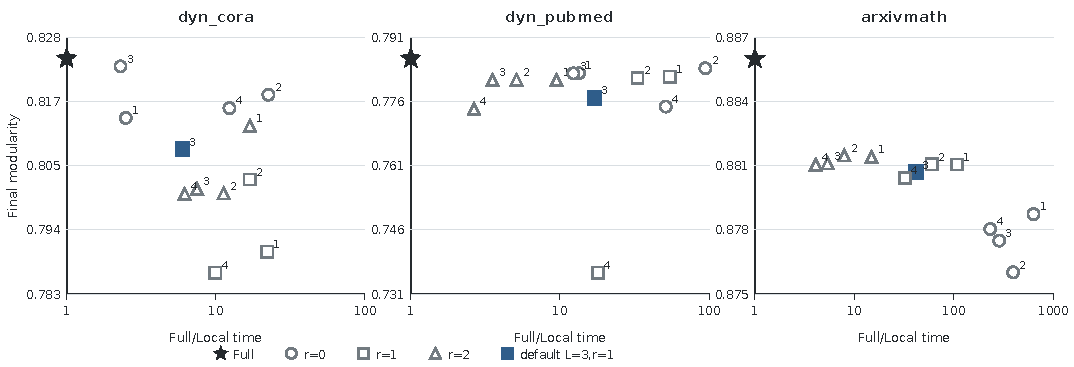
\includegraphics[width=0.98\textwidth]{topology_ablation.pdf}
\caption{Leiden quality--time grid for hierarchy depth
$L\in\{1,2,3,4\}$ and radius $r\in\{0,1,2\}$. Marker numbers show $L$;
color and shape show $r$; and the black line connects nondominated measured
points. The outlined orange square is the fixed $L=3,r=1$ configuration.
Non-default points are single runs; the default point averages five runs for
dyn\_pubmed and arxivmath and uses one run for dyn\_cora.}
\label{fig:topology}
\end{figure*}

No single $(L,r)$ setting dominates across the three datasets in
Fig.~\ref{fig:topology}. On dyn\_pubmed, $L=2,r=0$ reaches
$Q=\PubMedTopologyQ$ at \PubMedTopologySpeedup$\times$; on arxivmath,
$L=1,r=0$ reaches $Q=\ArxivTopologyQ$ at
\ArxivTopologySpeedup$\times$. Dyn\_cora follows a third pattern:
$L=3,r=0$ is closest to full modularity, whereas $L=2,r=0$ is the fastest
near-quality point. Increasing radius or hierarchy depth is therefore not a
monotone quality control. The $L=3,r=1$ setting was fixed in advance to provide
one common configuration across datasets, not selected as an empirical
optimum.

The resolution sweep in Table~\ref{tab:gamma} holds the remaining configuration fixed and evaluates
$\gamma\in\{0.5,1,2\}$ on the $999{:}50$ streams. ComNetX remains faster in
all six controls, by 41.6--161.8$\times$. The dyn\_pubmed modularity difference
ranges from $-0.004$ to $-0.053$, while the arxivmath difference stays between
$-0.004$ and $-0.013$. The acceleration therefore persists across the tested
resolution range, with graph-dependent quality sensitivity.

\begin{table*}[t]
\centering
\caption{Single-run Leiden resolution sweep; final modularity is reported as
full-snapshot/ComNetX.}
\label{tab:gamma}
\setlength{\tabcolsep}{5.0pt}
\small
\begin{tabular}{@{}lrrrrr@{}}
\toprule
\textbf{Dataset} & $\bm{\gamma}$ & \textbf{Updates} &
\textbf{Q} & $\bm{\Delta Q}$ & \textbf{Time ratio} \\
\midrule
dyn\_pubmed & 0.5 & 44 & 0.8362/0.8324 & $-0.0038$ & 44.8$\times$ \\
dyn\_pubmed & 1 & 44 & 0.7856/0.7592 & $-0.0265$ & 44.6$\times$ \\
dyn\_pubmed & 2 & 44 & 0.7373/0.6843 & $-0.0530$ & 41.6$\times$ \\
arxivmath & 0.5 & 50 & 0.9025/0.8982 & $-0.0043$ & 161.8$\times$ \\
arxivmath & 1 & 50 & 0.8859/0.8759 & $-0.0100$ & 140.3$\times$ \\
arxivmath & 2 & 50 & 0.8665/0.8540 & $-0.0125$ & 135.9$\times$ \\
\bottomrule

\end{tabular}
\end{table*}

\subsubsection{Effect of Edge Direction}
The main tables symmetrize the topology. Table~\ref{tab:directed} retains the
stored direction for a separate Leiden control on the two larger short streams.
With the stored edge directions retained, ComNetX is 14.0$\times$ faster on
dyn\_pubmed and 38.4$\times$ faster on arxivmath, with the quality differences
reported in Table~\ref{tab:directed}. These two controls show that the measured
speedup is not caused solely by symmetrizing the input graphs.

\begin{table*}[t]
\centering
\caption{Direction-preserving Leiden control; quality and time values are
full-snapshot/ComNetX.}
\label{tab:directed}
\setlength{\tabcolsep}{5.0pt}
\small
\begin{tabular}{@{}lrrrr@{}}
\toprule
\textbf{Dataset} & \textbf{Q} & \textbf{NMI} &
\textbf{T (s)} & \textbf{Time ratio} \\
\midrule
dyn\_pubmed & 0.788/0.768 & 0.208/0.199 & 4.990/0.356 & 14.0$\times$ \\
arxivmath & 0.886/0.880 & 0.415/0.404 & 108.8/2.834 & 38.4$\times$ \\
\bottomrule

\end{tabular}
\end{table*}

\subsubsection{Effect of Feature Representation}
Table~\ref{tab:features} reports the feature ablation with five internal runs
of $T=10$ per S$^2$CAG invocation. The $999{:}100$ construction yields ten
nonempty updates on dyn\_cora and 44 on dyn\_pubmed; each cell reports final
$Q$, cumulative measured processing time, and final NMI.

\begin{table*}[t]
\centering
\caption{S$^2$CAG feature sensitivity; each cell reports final modularity,
cumulative measured processing time in seconds, and final NMI.}
\label{tab:features}
\setlength{\tabcolsep}{5.0pt}
\small
\begin{tabular}{@{}lcc@{}}
\toprule
\textbf{Variant} & \textbf{dyn\_cora (10 updates)} &
\textbf{dyn\_pubmed (44 updates)} \\
\midrule
Full, dataset features & $0.691$/35.71/0.437 & $0.624$/372.4/0.202 \\
ComNetX, dataset features & $0.788$/6.822/0.463 & $0.532$/36.54/0.180 \\
Full, random features & $-0.001$/13.02/0.023 & $-0.002$/92.18/0.000 \\
ComNetX, random features & $0.784$/4.669/0.462 & $0.534$/25.68/0.186 \\
Full, one-hot features & $0.751$/43.96/0.360 & $0.528$/8568.1/0.059 \\
ComNetX, one-hot features & $0.779$/7.251/0.452 & $0.518$/195.6/0.182 \\
\bottomrule

\end{tabular}
\end{table*}

Dataset features yield the highest local dyn\_cora modularity and NMI in this
fixed-budget control. Random features yield near-zero modularity for both full
calls ($-0.001$ and $-0.002$), yet the corresponding ComNetX rows remain close
to the local dataset-feature rows: 0.784 versus 0.788 on dyn\_cora and 0.534
versus 0.532 on dyn\_pubmed. One-hot features produce the highest full
dyn\_cora modularity but increase full dyn\_pubmed measured processing time
from 372.4 s to 8568.1 s. Each ComNetX call combines the selected features with
graph topology; the maintained hierarchy determines the contracted atoms but
is not supplied to S$^2$CAG as an initial partition. The interaction between
feature mode and local/full input is specific to these contracted graphs,
fixed budgets, and cluster-count rules; it does not imply that random features
generally substitute for attributes.

Across the measured controls, neither radius and depth nor feature
representation follows a transferable ordering: the preferred $(L,r)$ setting
depends on the graph, and the feature response changes between full and
contracted calls.

\subsection{Quality and Processing Time over 500 Updates (RQ5)}

The 500-update runs retain a substantial time advantage but reveal cumulative
quality differences. On dyn\_pubmed, ComNetX is 15.9$\times$ faster, while
final modularity changes from 0.784 to 0.748 and NMI from 0.208 to 0.153. On
arxivmath, the time ratio remains \ArxivLongSpeedup$\times$, with final
modularity \ArxivLongLocalQ\ versus \ArxivLongFullQ\ and NMI
\ArxivLongLocalNMI\ versus \ArxivLongFullNMI. Table~\ref{tab:long} and
Fig.~\ref{fig:long} give both trajectories. Dyn\_pubmed uses the artificial
edge order, whereas arxivmath uses timestamps; the figure reports per-update
modularity differences and cumulative processing-time ratios for Leiden.

\begin{table*}[t]
\centering
\caption{Quality and measured processing time after 500 updates. Values are
baseline/ComNetX; the time ratio is baseline time divided by ComNetX time.}
\label{tab:long}
\setlength{\tabcolsep}{4.8pt}
\small
\begin{tabular}{@{}llcccc@{}}
\toprule
\textbf{Dataset} & \textbf{Backend} & \textbf{Q} & \textbf{NMI} &
\textbf{T (s)} & \textbf{Time ratio} \\
\midrule
dyn\_pubmed & Leiden & 0.784/0.748 & 0.208/0.153 & 315.4/19.78 & 15.95$\times$ \\
dyn\_pubmed & DF-Leiden & 0.762/0.715 & 0.195/0.138 & 6.234/5.945 & 1.05$\times$ \\
arxivmath & Leiden & 0.887/0.874 & 0.427/0.355 & 7201.7/235.8 & 30.54$\times$ \\
arxivmath & DF-Leiden & 0.855/0.869 & 0.388/0.335 & 198.9/26.84 & 7.41$\times$ \\
\bottomrule

\end{tabular}
\end{table*}

\begin{figure*}[t]
\centering
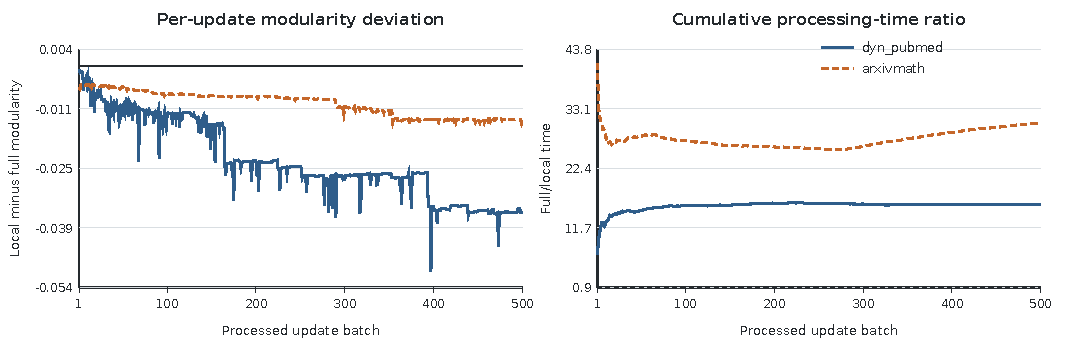
\includegraphics[width=0.97\textwidth]{long_horizon.pdf}
\caption{Leiden trajectories over 500 updates. Left: per-batch
ComNetX-minus-full modularity, where negative values favor the full partition. Right:
cumulative full/ComNetX processing-time ratio, where values above one favor
ComNetX.}
\label{fig:long}
\end{figure*}

Across the 500 dyn\_pubmed updates, the mean local-minus-full modularity
difference is $-0.0232$, and its minimum is $-0.0500$ at update 397. For
arxivmath, the corresponding values are $-0.00922$ and $-0.01430$ at update
373. Arxivmath therefore remains within a narrower modularity band, whereas
dyn\_pubmed exhibits a wider gap despite preserving a time advantage.
Sustained time gains therefore coexist with markedly different drift profiles.

With DF-Leiden as the backend, the ComNetX method is close to the native stream
time on dyn\_pubmed and 7.4$\times$ faster on arxivmath. On arxivmath, the two
metrics rank the partitions differently: ComNetX has higher modularity but
lower agreement with the external labels.

\subsection{Effect of the Number and Placement of Updated Edges (RQ5)}

Update placement changes the break-even point even at a fixed batch size. At
1450 changed edges per update, ComNetX is slower for every random and
hub-centered seed but remains faster for every community-internal seed.
Table~\ref{tab:dsbm} gives the mean paired time ratio and worst local-minus-full
quality difference over five seeds; Fig.~\ref{fig:dsbm} shows the paired
speedup ranges.

\begin{table}[t]
\centering
\caption{DSBM stress test over 99 insertion batches and five seeds; $\pm$ is
the sample standard deviation of paired speedup across seeds.}
\label{tab:dsbm}
\setlength{\tabcolsep}{2.4pt}
\scriptsize
\begin{tabular}{@{}llrrr@{}}
\toprule
\textbf{Edges/update} & \textbf{Update type} & \textbf{Mean speedup} &
\textbf{Worst $\Delta Q$} & \textbf{Worst $\Delta$NMI} \\
\midrule
290 & random & 3.34 $\pm$ 0.025 & $-0.0031$ & $-0.0158$ \\
290 & hub-centered & 1.53 $\pm$ 0.012 & $-0.0022$ & $-0.0135$ \\
290 & community-internal & 4.29 $\pm$ 0.073 & $-0.0102$ & $-0.0481$ \\
1450 & random & 0.89 $\pm$ 0.002 & $-0.0049$ & $-0.0329$ \\
1450 & hub-centered & 0.85 $\pm$ 0.003 & $-0.0050$ & $-0.0286$ \\
1450 & community-internal & 1.13 $\pm$ 0.011 & $-0.0088$ & $-0.0561$ \\
\bottomrule

\end{tabular}
\end{table}

\begin{figure}[t]
\centering
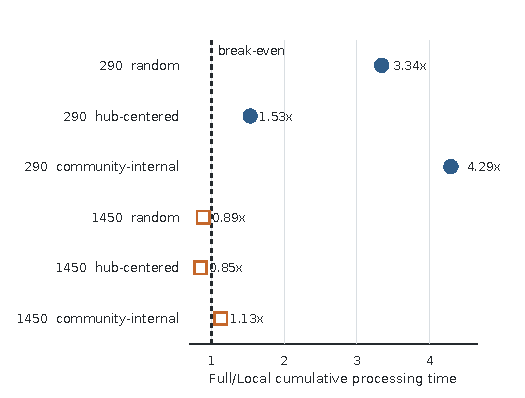
\includegraphics[width=0.98\columnwidth]{dsbm_speedup.pdf}
\caption{Mean and seed range of full/ComNetX cumulative measured processing time
in the DSBM stress test. Filled markers denote 290 changed edges per
update; open markers denote 1450.}
\label{fig:dsbm}
\end{figure}

At 290 changed edges per update, all 15 paired seed runs are faster with
ComNetX, and the three update types yield mean speedups from 1.53$\times$ to
4.29$\times$. At 1450 edges, the random and hub-centered mean time ratios are
\DSBMHighRandomSpeedup$\times$ and
\DSBMHighHubSpeedup$\times$, whereas the community-internal mean speedup is
1.13$\times$. Across all conditions, the worst absolute modularity difference
is 0.0102. At a fixed batch size, edge placement materially changes the
observed break-even behavior.

\subsection{Practical Implications}

ComNetX is useful when the wrapped detector is expensive enough for graph
reduction to repay local preprocessing. The dyn\_pubmed DF-Leiden result gives
the clearest counterexample: a persistent native stream takes 0.106 s, whereas
ComNetX with fresh quotient calls takes 0.243 s. The number of changed edges is
also insufficient. With 1450 changed edges per batch in the DSBM experiment,
ComNetX is slower for random and hub-centered updates but remains faster for
community-internal updates.

Candidate deployment signals identified by the analysis are the closed-scope
and quotient sizes relative to the cost of a full detector call, rather than
merely the number of changed edges. The quantities $h_\ell$, $e_\ell$,
$k_\ell$, and $q_\ell$ are available during an update and could support a policy that
switches between local and full processing; such a controller is not
implemented or evaluated here. Runtime-based switching would not by itself
control partition quality: the 500-update runs retain a time advantage while
ending with nonzero modularity and NMI gaps.

\section{Reproducibility and Scope of the Results}
\label{sec:reproducibility}

All quantitative tables and figures are generated from archived measurement
records rather than transcribed manually. The accompanying program verifies
the required experiment keys, update counts, graph representations,
repetitions, and paired DSBM seeds before emitting the LaTeX tables and vector
figures. The ComNetX implementation is available at
\url{https://github.com/mpailab/comnetx}. The source package accompanying this
manuscript contains the validated records, configurations, generator, and
article assets; dataset sources are identified in
Section~\ref{sec:experiments}.

The evaluation targets fixed-vertex edge-insertion streams with fixed
attributes. Four real-graph benchmarks use artificial edge orders, while
patent and arxivmath use timestamps. The two 500-update experiments each use
one retained window: dyn\_pubmed follows its artificial order and arxivmath
follows timestamps. Repeated real-graph runs quantify timing repeatability on
the same streams; the DSBM suite supplies five independent graph seeds per
condition. Most non-default topology-grid points are single runs, and the
S$^2$CAG experiments use the fixed budgets and cluster-count rules stated in
Section~\ref{sec:experiments}. Accordingly, the results apply to the measured
fixed edge-insertion streams and configurations; deletion streams, arriving
vertices, changing node features, and independent real-data windows remain
outside the empirical scope.

\section{Conclusion}
\label{sec:conclusion}

ComNetX addresses the gap between repeated full-snapshot optimization and
detector-specific dynamic algorithms. It includes all vertices of each touched
pre-update community in the reassignment scope, represents hierarchy-defined
groups as weighted supernodes, and lifts the backend partitions to the original
vertices while preserving hierarchy nesting. This construction leaves the
backend implementation unchanged and separates the vertices allowed to change
from the graph presented to the detector. It does not make local and
full-snapshot optimization equivalent: contracted atoms restrict admissible
splits, and the induced working graph omits boundary interactions. The scoped
quotient identity and boundary decomposition make that distinction explicit.

Under the reported timing convention, ComNetX with Leiden is faster on all six
short streams; on arxivmath, cumulative measured processing time falls from
149.1 s to 3.559 s
while final modularity changes from \ArxivShortFullQ\ to \ArxivShortLocalQ.
The 500-update arxivmath trajectory retains a \ArxivLongSpeedup-fold time
advantage with a final modularity difference of \ArxivLongQGap. The component
trajectories are consistent with complementary roles: omitting closure
coincides with lower final modularity, whereas omitting contraction sharply
enlarges the backend graph and measured profile time.

Empirically, native DF-Leiden is faster on dyn\_pubmed, and high-rate random or
hub-centered DSBM updates favor full recomputation. Analytically, a touched
scope may span the graph and require up to $L$ full-size backend calls. ComNetX
is therefore most appropriate when a compatible detector lacks an effective
native update path and the touched communities admit compact quotients;
otherwise, full recomputation or a specialized dynamic algorithm remains
preferable.

\appendices

\section{Boundary Term for Modularity}
\label{app:boundary}

To relate scoped and full-graph modularity, assume $A_{ij}\ge0$,
$W=\sum_{i,j}A_{ij}>0$, and
$\gamma\ge0$. Let $U=U_t^\ell$,
$W_U=\sum_{i,j\in U}A_{ij}>0$, and let $z$ be an inside partition whose labels
are disjoint from the fixed outside partition. Let $C_z$ combine $z$ with that
retained outside partition. For each inside block $a$, let $x_a$ and $y_a$ be
its outgoing and incoming degree within $U$, and define its boundary degrees by
\begin{equation}
p_a=\sum_{i\in a,j\notin U}A_{ij},\qquad
q_a=\sum_{i\notin U,j\in a}A_{ij}.
\label{eq:boundary_degrees}
\end{equation}

\noindent\textbf{Proposition A.1 (exact boundary decomposition):} If
$K_{V\setminus U}$ is the full-modularity contribution independent of $z$,
direct substitution in \eqref{eq:modularity} gives
\begin{equation}
\begin{aligned}
D(z)={}&Q_\gamma(\bm A,C_z)-K_{V\setminus U}
-\frac{W_U}{W}Q_\gamma(\bm{A}[U],z)\\
={}&\frac{\gamma}{W^2}\left[
\frac{W-W_U}{W_U}\sum_a x_ay_a\right.\\
&\left.\hspace{12mm}-\sum_a(x_aq_a+y_ap_a+p_aq_a)\right].
\end{aligned}
\label{eq:boundary_mismatch}
\end{equation}
The internal-edge term is unchanged; the mismatch consists of the
global-versus-local null-model normalization and the boundary degrees.

Write $\beta_{\mathrm{out}}=\sum_a p_a$ and
$\beta_{\mathrm{in}}=\sum_a q_a$. Nonnegativity gives
\begin{equation}
-B_-\le D(z)\le B_+,
\label{eq:boundary_interval}
\end{equation}
where
\begin{equation}
\begin{aligned}
B_+&=\frac{\gamma}{W^2}W_U(W-W_U),\\
B_-&=\frac{\gamma}{W^2}\left[
W_U(\beta_{\mathrm{out}}+\beta_{\mathrm{in}})
+\beta_{\mathrm{out}}\beta_{\mathrm{in}}\right].
\end{aligned}
\label{eq:boundary_bounds}
\end{equation}
For example, $\sum_a x_ay_a\le W_U^2$,
$\sum_a x_aq_a\le W_U\beta_{\mathrm{in}}$, and the analogous bounds for the
remaining terms give \eqref{eq:boundary_interval}.

For one fixed family $\mathcal{S}$ of partitions respecting the declared
atoms, define $F(z)=Q_\gamma(\bm A,C_z)-K_{V\setminus U}$ and
$L(z)=(W_U/W)Q_\gamma(\bm{A}[U],z)$. If $z_U$ maximizes $L$ and $z_G$
maximizes $F$ over $\mathcal{S}$, then
\begin{equation}
0\le F(z_G)-F(z_U)\le B_-+B_+.
\label{eq:restricted_loss}
\end{equation}
This bound compares exact optima only within the same atom-respecting candidate
family; it does not bound loss against an unrestricted full-graph optimum or
certify the output of a heuristic backend.

\section{Implementation Cost and an Indexed Alternative}
\label{app:implementation_cost}

The current PyTorch implementation symmetrizes and traverses the resident
adjacency for neighborhood expansion. At every hierarchy level, it scans the
global label and edge arrays, restricts the working graph, compacts group
labels, contracts sparse edges, optionally aggregates features, and invokes
the backend. Filtering the resident adjacency independently for every
immutable scope produces the $Ls_t$ term in
\eqref{eq:full_scan_lower}: quotient graphs can be small while front-end memory
traffic remains graph-wide.

The implementation stores all immutable Boolean closures and processes levels
sequentially. Let $M_{\mathrm{SpMM},\ell}$ and $M_{\mathcal B,\ell}$ denote
sparse-product and backend workspace. Its additional space is conservatively
bounded by
\begin{equation}
\begin{aligned}
M_{\mathrm{extra}}=O\!\Bigl(Ln+\max\bigl\{&s_t+n,\\
&\max_\ell\bigl[e_\ell+h_\ell+q_\ell+M_{\mathrm{feat},\ell}\\
&\quad{}+M_{\mathrm{SpMM},\ell}
+M_{\mathcal B,\ell}\bigr]\bigr\}\Bigr).
\end{aligned}
\label{eq:current_space}
\end{equation}
An indexed realization can store immutable scopes as vertex lists, replacing
the $Ln$ closure masks in additional workspace by $\sum_\ell h_\ell$; the
resident adjacency, hierarchy, feature, and backend-workspace terms remain.
With adjacency lists, a community-to-members index, and indexed incident edges,
let $\mu_r$ be the support-edge volume visited by the radius search and
$\rho_\ell$ the incident-edge volume inspected at level $\ell$. Let $f_\ell$
be the selected feature entries ($f_\ell=h_\ell d$ for dense scoped features).
Including the
cost $T_{\mathrm{index}}(\bm\Delta_t)$ of maintaining these indices, expected
hash-based aggregation gives the output-sensitive bound
\begin{equation}
\begin{aligned}
T_{\mathrm{indexed}}=T_{\mathrm{index}}(\bm\Delta_t)+O\!\Biggl(&\mu_r+
\sum_{\ell=0}^{L-1}\bigl[h_\ell+\rho_\ell+q_\ell+f_\ell\\
&{}+\overline T_{\mathcal B}(k_\ell,q_\ell,d)\bigr]\Biggr).
\end{aligned}
\label{eq:indexed_cost}
\end{equation}
This alternative removes mandatory full scans only in local cases; it retains
the graph-wide worst case when the reached regions span the snapshot.

\section*{Acknowledgment}
OpenAI Codex was used to assist with language editing and structural revision
of the Abstract, Introduction, Method, Results and Discussion, and Conclusion;
with consistency checks against the archived measurements; and with preparation
of vector-figure code. The authors reviewed and revised all resulting text,
code, figures, citations, and numerical claims and take responsibility for the
article's content and conclusions.

\bibliographystyle{IEEEtran}
\bibliography{references}

\begin{IEEEbiographynophoto}{Aleksandr Konovalov}
received the Specialist degree from the Faculty of Mechanics and Mathematics,
Lomonosov Moscow State University, Moscow, Russia, in 2013, and the Candidate
of Physical and Mathematical Sciences degree in 2018. He is currently a Junior
Researcher with Lomonosov Moscow State University. His research interests
include constructive mathematical logic, graph neural networks, and dynamic
community detection.
\end{IEEEbiographynophoto}

\begin{IEEEbiographynophoto}{Anna Uporova}
is currently pursuing the Specialist degree with the Faculty of Mechanics and
Mathematics, Lomonosov Moscow State University, Moscow, Russia. Her research
interests include dynamic graphs, community detection, and graph neural
networks.
\end{IEEEbiographynophoto}

\begin{IEEEbiographynophoto}{Alexander Drobyshev}
is currently a postgraduate student with the Chair of Mathematical Theory of
Intelligent Systems, Faculty of Mechanics and Mathematics, Lomonosov Moscow
State University, Moscow, Russia. His research interests include
Boolean-network dynamics, limit cycles, computational complexity, and dynamic
graph algorithms.
\end{IEEEbiographynophoto}

\begin{IEEEbiographynophoto}{Iaroslav Egorov}
is affiliated with the AI Research Center, Lomonosov Moscow State University,
Moscow, Russia. His recent work includes scalable dynamic community detection.
\end{IEEEbiographynophoto}

\begin{IEEEbiographynophoto}{Grigoriy Bokov}
received the Candidate of Physical and Mathematical Sciences degree in 2014.
He is currently the Director of the AI Research Center, Lomonosov Moscow State
University, Moscow, Russia, and an Associate Professor and the Head of the
Laboratory of Mathematical Problems of Artificial Intelligence at the Faculty
of Mechanics and Mathematics. His research interests include logical calculi,
functional systems, automata, machine-learning algorithms, optimization, and
large dynamic graphs.
\end{IEEEbiographynophoto}

\EOD
\end{document}
